\documentclass[12pt]{article}

\usepackage{a4wide} % уменьшает поля
\usepackage[utf8]{inputenc}
\usepackage[russian]{babel} % включает русский язык
\usepackage{graphicx} % позволяет подключить .eps - файлы
\usepackage{amsmath}
\usepackage{amsthm} % теоремы от AMS
\usepackage{amssymb} % для работы с математическими R и проч.
\usepackage{floatrow}
\usepackage{mathrsfs}
\usepackage[section]{placeins}
\usepackage{indentfirst} % абзац после заголовка
\usepackage{misccorr} % точки в заголовках

%\graphicspath{{pics/}}


%\newtheoremstyle{rusdef}
%  {3pt}% measure of space to leave above the theorem. E.g.: 3pt
%  {3pt}% measure of space to leave below the theorem. E.g.: 3pt
%  {\itshape}% name of font to use in the body of the theorem
%  {\parindent}% measure of space to indent
%  {\bfseries}% name of head font
%  {.}%
%  {.5em}%
%  {}


\theoremstyle{rusdef}
\renewcommand\qedsymbol{$\blacksquare$}
\newtheorem{remark}{Замечание}
\newtheorem{theorem}{Теорема}
\newtheorem{definition}{Определение}
\newtheorem{proposition}{Утверждение}

\newcommand*{\hm}[1]{#1\nobreak\discretionary{}{\hbox{$\mathsurround=0pt #1$}}{}}
\newcommand{\scalar}[2]{\left<#1,#2\right>}
\newcommand{\const}{\ensuremath{\operatorname{const}}}
\newcommand{\sgn}{\ensuremath{\operatorname{sgn}}}
\renewcommand{\d}[1]{\ensuremath{\operatorname{d}\!{#1}}}
\newcommand\abs[1]{\left\lvert #1 \right\rvert} % модуль
\newcommand\brackets[1]{\left( #1 \right)} % скобки
\newcommand{\R}{\ensuremath{\mathbb{R}}} % R - мн-во вещественных чисел
\newcommand{\N}{\ensuremath{\mathbb{N}}} % N - мн-во натуральных чисел
\newcommand{\Z}{\ensuremath{\mathbb{Z}}} % Z - мн-во целых чисел
\renewcommand{\C}{\ensuremath{\mathbb{C}}} % C - мн-во комплексных чисел
\newcommand{\E}{\ensuremath{\mathcal{E}}} % E --- эллипсоид
\newcommand{\norm}[1]{\left\lVert #1 \right\rVert} % норма
\DeclareMathOperator*{\thus}{\Rightarrow} % следствие с возможностью использовать limits
\DeclareMathOperator*{\tolim}{\to} % стремление с возможностью использовать limits
\DeclareMathOperator*{\Argmax}{Argmax} % Argmax с возмножностью использовать limits
\DeclareMathOperator{\rank}{rank} % ранг
\DeclareMathOperator{\e}{e} % экспонента

\newcommand{\rpm}{\sbox0{$1$}\sbox2{$\scriptstyle\pm$}
	\raise\dimexpr(\ht1)/2\relax\box2 } % крутой плюс-минус

\begin{document}
	\thispagestyle{empty}
	
	\begin{center}
		\ \vspace{-3cm}
		
		\includegraphics[width=0.5\textwidth]{msu.eps}\\
		
		{\scshape Московский Государственный Университет имени М.~В.~Ломоносова}\\
		Факультет Вычислительной Математики и Кибернетики\\
		Кафедра Системного Анализа
		\vfill
		
		{\LARGE Отчёт по заданию курса <<Суперкомпьютерное моделирование и технологии>>}
		\vspace{.5cm}
		
	\end{center}
	
	\vspace{1cm}
	
	\begin{flushright}
		\large
		\textit{Студент 615 группы}\\
		В.~С.~Терёшин\\
		
	\end{flushright}
	
	\vfill
	
	\begin{center}
		{\large
			Москва, 2016г.}
	\end{center}
	
	\newpage
	\tableofcontents
	\newpage
	
	\section{Постановка задачи}
	
	В прямоугольной области $\Pi = [A_1,A_2] \times [B_1,B_2]$ требуется найти дважды дифференцируемую функцию $u=u(x,y)$, удовлетворяющую дифференциальным уравнению
	$$-\Delta u=F(x,y),\;A_1<x<A_2,\;B_1<y<B_2$$
	и дополнительному условию $u(x,y)=\phi(x,y)$ во всех граничных точках $(x,y)$ прямоугольника.

	Оператор Лапласа $\Delta$ определяется равенством $\Delta u= \tfrac{\delta^2 u}{\delta^2 x} + \tfrac{\delta^2 u}{\delta^2 y}$.
	
	Функции $F(x,y)$ и $\phi(x,y)$ определены следующим образом:
	\begin{gather}
	F(x,y)=(x^2+y^2)\sin(xy), \notag \\
	\phi(x,y)=1+\sin(xy), \notag \\
	A_1=-2,\;A_2=2,\;B_1= -2,B_2=2. \notag
	\end{gather}
	
	
	\section{Численный алгоритм решения}
	
	В расчётной области $\Pi$ определяется прямоугольная сетка $$\omega_h=\left\{x_i,y_j,i=0,1,\ldots,N_1,j=0,1,2,\ldots,N_2\right\},$$
	где $A_1=x_0<x_1<x_2<\ldots<x_{N_1}=A_2$ --- разбиение $[A_1,A_2]$ оси $OX$,
	а $B_1=y_0<y_1<y_2<\ldots<y_{N_2}=B_2$ --- разбиение $[B_1,B_2]$ оси $OY$.
	Через $\omega_h$ обозначим множество внтуренних, а через $\gamma_h$ --- множество граничных узлов сетки. Пусть.
	Рассмотрим линейное пространство $H$ функций, заданных на сетке. Будем считать, что в этом пространстве заданы скалярное произведение и евклидова норма
	$$(u,v) = \sum\limits_{i=1}^{N_1-1} \sum\limits_{j=1}^{N_2-1} \hat{h}_i^{(1)} \hat{h}_j^{(2)} u_{ij}v_{ij}.$$
	
	Где $u_{ij}=u(x_i,y_j)$, $v_{ij}=v(x_i,y_j)$ --- любые функции из пространсва $H$.
	Для аппроксимации уравнения Пуассона используется пятиточечный разностный оператор Лапласа, который можно определить во внутренних узлах сетки следующим равенством:
	$$
	-\Delta_h p_{ij}= \tfrac{1}{h_i^{(1)}}\left( \frac{p_{ij} - p_{i-1,j}}{h_{i-1}^{(1)}} -\frac{p_{i+1,j} - p_{ij}}{h_i^{(1)}} \right) + \tfrac{1}{h_j^{(2)}}\left( \frac{p_{ij} - p_{i,j-1}}{h_{j-1}^{(2)}} -\frac{p_{i,j+1} - p_{ij}}{h_j^{(2)}} \right).
	$$
	Предполагается, что функция $p=p(x_i,y_j)$ определена во всех точках сетки. Приближенным решением искомой задачи Дирихле называется функция $p=p(x_i,y_j)$, удовлетворяющая уравнениям
	\begin{gather}
	-\Delta_h p_{ij}=F(x_i,y_j),\; x_i,y_j \in \omega_h, \notag \\
	p_{ij} = \phi(x_i,y_j), \; x_i,y_j\in \gamma_h. \notag
	\end{gather}
	
	
	\section{Решение системы линейных алгебраических уравнений}
	
	Приближенное решение СЛАУ получается итерационным методом сопряженных градиентов.
	
	Первая итерация метода выполняется согласно методу скорейшего спуска, а процесс выполнения последующих итераций отличается.
	
	Начальное приближение $p_{ij}(0)= \phi(x_i,y_j), \; x_i,y_j \in \gamma_h$, во внутренних узлах сетки первое приближение осуществляется любыми числами (в нашем случае все внутренние узлы сетки инициализированы значением $0$).
	
	Метод является одношаговым, первая итерация $p_{ij}^{(1)}$ вычисляется по итерации $p_{ij}^{(0)}$ согласно следующим равенствам:
	$p_{ij}^{(1)}=p_{ij}^{(0)}-\tau^{(k+1)}r_{ij}^{(0)}$.
	Невязка определяется согласно формуле
	$$
	r_{ij}^{(k)}= -\Delta_h p_{ij}^{(k)}-F(x_i,y_j), \; (x_i,y_j) \in \omega_h,
	$$
	$$
	r_{ij}^{(k)}=0, \; (x_i,y_j)\in \gamma_h.
	$$
	Итерационный параметр:
	$\tau^{(k+1)}= (r^{(k)},r^{(k)})(-\Delta_h r^{(k)},r^{(k)})$.
	
	
	Последующие итерации вычисляются по методу сопряженных градиентов, определенный формулами:
	\begin{gather}
	p_{ij}^{(k+1)}=p_{ij}^{(k)}-\tau^{(k+1)} g_{ij}^{(k)}, \notag \\
	\tau^{(k+1)}= (r^{(k)},g^{(k)})(-\Delta_h g^{(k)},g^{(k)}), \notag \\
	g_{ij}^{(k)}=r_{ij}^{(k)}-a^k g_{ij}^{(k-1)}, k=1,2,\ldots, \notag \\
	g_{ij}^{(0)}=r_{ij}^{(0)}, \notag \\
	a^k= (-\Delta_h r^{(k)},g^{(k-1)})(-\Delta_h g^{(k-1)},g^{(k-1)}). \notag
	\end{gather}
	Итерационный процесс останавливается, как только максимум-норма разности приближенных решений на итерациях $(n+1)$ и $n$ становится меньше заранее заданного числа $\varepsilon$, равного $10^{-4}$.
	
	
	\section{Описание работы программы}
	\begin{enumerate}
	\item Принимает на вход: MPI параметры, определяющие число процессов, OpenMP параметры, определяющие число потоков внутри процесса, задан размер сетки по осям Ох и Oy; задано условие на погрешность;
	\item Обмен между процессами осуществляется c помощью функций \texttt{MPI\_Bcast}, \texttt{MPI\_Reduce}, \texttt{MPI\_Allgatherv};
	\item Из средств OpenMP используются конструкции для создания потоков (директива parallel) на одном вычислительном узле.
	\end{enumerate}
	
	\section{Время работы программы}
	Результаты работы на ПВС «Ломоносов»:
	
	\begin{tabular}{ c c c c }
		\hline
		Число процессоров & Размер сетки & Время работы & Ускорение \\
		\hline
		8 & $1000\times1000$ & 23.0124 & \\
		16 & $1000\times1000$ & 15.1178 & 1.5222 \\
		32 & $1000\times1000$ & 8.9701 & 1.6853 \\
		128 & $1000\times1000$ & 3.0169 & 2.9732 \\
		8 & $2000\times2000$ & 149.8731 & \\
		16 & $2000\times2000$ & 86.3512 & 1.7356 \\
		32 & $2000\times2000$ & 47.1164 & 1.8327 \\
		128 & $2000\times2000$ & 12.5504 & 3.7541 \\
		\hline
	\end{tabular}\newline\newline
	
	Результаты работы на ПВС IBM BG/P без OpenMP:
	
	\begin{tabular}{ c c c c }
		\hline
		Число процессоров & Размер сетки & Время работы & Ускорение \\
		\hline
		128 & $1000\times1000$ & 20.9734 & \\
		256 & $1000\times1000$ & 10.7882 & 1.9441 \\
		512 & $1000\times1000$ & 5.9136 & 1.8243 \\
		128 & $2000\times2000$ & 127.7592 & \\
		256 & $2000\times2000$ & 64.0003 & 1.9962 \\
		512 & $2000\times2000$ & 36.7831 & 1.7399 \\
		\hline
	\end{tabular}\newline\newline
	
	Результаты работы на ПВС IBM BG/P с OpenMP:

	\begin{tabular}{ c c c c }
		\hline
		Число процессоров & Размер сетки & Время работы & Ускорение \\
		\hline
		128 & $1000\times1000$ & 10.5649 & \\
		256 & $1000\times1000$ & 5.9375 & 1.7793 \\
		512 & $1000\times1000$ & 2.9994 & 1.9795 \\
		128 & $2000\times2000$ & 70.2247 & \\
		256 & $2000\times2000$ & 36.1414 & 1.9430 \\
		512 & $2000\times2000$ & 18.4670 & 1.9570 \\
		\hline
	\end{tabular}\newline\newline

	\section{Сравнение с точным решением}
	
	Точное решение (найдено подбором): $u(x,y)=1+\sin(xy)$.
	
	Красная поверхность: точное решение; зелёная --- полученное с помощью численного метода.

	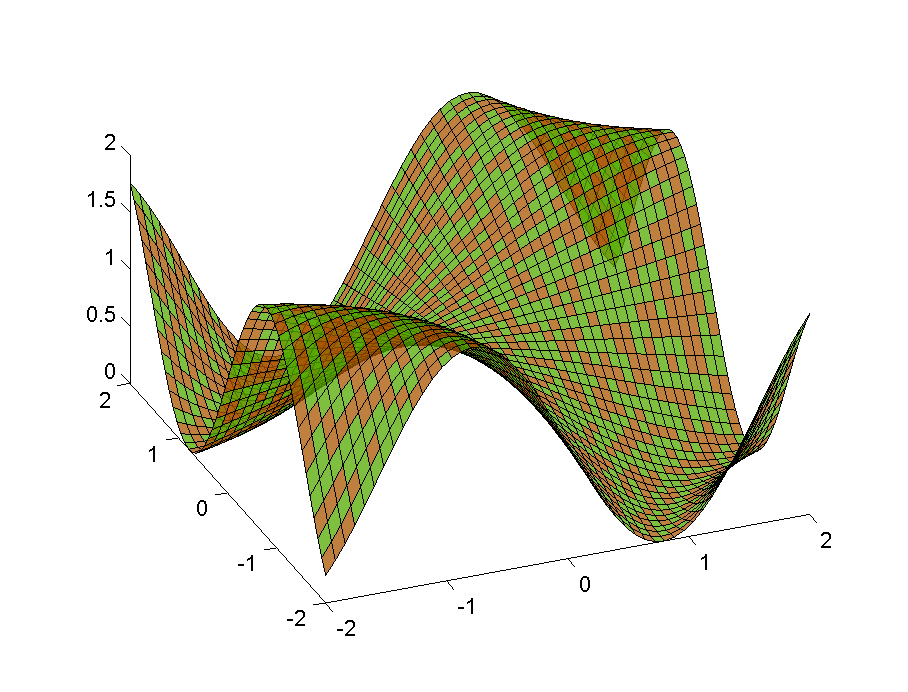
\includegraphics{plot.eps}\\
	
\end{document}